
%(BEGIN_QUESTION)
% Copyright 2010, Tony R. Kuphaldt, released under the Creative Commons Attribution License (v 1.0)
% This means you may do almost anything with this work of mine, so long as you give me proper credit

A trend recorder is connected to a {\it current transformer}, which is clamped around one of the power conductors leading to the three-phase electric motor powering a utility elevator.  As the elevator lifts a load, the motor's torque translates into line current which is measured and plotted by the trend recorder.  The heavier the load lifted, the more torque output by the motor, and the more current drawn by the motor.

$$\includegraphics[width=15.5cm]{i01613x01.eps}$$

Calculate the approximate amount of {\it work} done by this elevator (in the unit of joules), knowing that the power of a three-phase electric motor is equal to line voltage (480 volts) times line current (graphed) times the square root of 3, and also knowing that one {\it watt} is equivalent to one {\it joule} of work performed each {\it second} (watts = joules per seconds):

$$P = V_{line} I_{line} \sqrt{3}$$

Also, explain the significance of the ``hump'' appearing mid-way in the elevator's travel.  What does this odd shape suggest about the elevator?

\vfil 

\underbar{file i01613}
\eject
%(END_QUESTION)





%(BEGIN_ANSWER)

This is a graded question -- no answers or hints given!

%(END_ANSWER)





%(BEGIN_NOTES)

The units of measurement in this problem tell us what type of calculus operation we must apply to it.  Since motor power (which may be interpreted directly from the current plotted on the graph, given a constant line voltage) is measured in {\it watts}, which is {\it joules of energy per second}, and time of course may be measured in {\it seconds}, we need to choose a mathematical operation to cancel out the time (seconds) and leave us with energy (joules).  Obviously, we must use {\it multiplication} to allow seconds to cancel joules per second to arrive at joules:

$$\left( {[\hbox{joules}] \over [\hbox{seconds}]} \right) \left( {[\hbox{seconds}] \over 1} \right)$$

Since we know multiplication is associated with the calculus operation of {\it integration}, we can tell that work (energy) will be the integral of power with respect to time:

$$W = \int P \> dt$$

The graphical interpretation of integration is the geometric area bound by the function.  Thus, we will approximate the amount of area found between the current plot and zero.  One way to do this is to integrate current with respect to time, yielding a result in the unit of {\it amp-seconds}.  We can then multiply this integrated line current by line voltage (480 VAC) and the square-root of time to get an answer in watt-seconds, which is the same thing as joules:

$$[\hbox{Amp-seconds}] = \int I \> dt$$

$$\includegraphics[width=15.5cm]{i01613x02.eps}$$

An integrated current value of 233 amp-seconds multiplied by $480 \sqrt{3}$ is equal to approximately 193,700 joules of work.

\vskip 10pt

The ``hump'' suggests mechanical friction at one point along the elevator's travel.  This is abnormal, and should be looked in to by the appropriate maintenance staff.

%INDEX% Mathematics, calculus: integral (work)

%(END_NOTES)


